The proposed flatwise-wound transformer and its edgewise equivalent are simulated in Ansys Electronics using the Maxwell and Icepak solvers to check if the transformer design results in an electrically and thermally viable transformer. This chapter details the simulation conditions to carry out this evaluation. The results of the electromagnetic, electrostatic, and thermal simulations are described. Moreover, a geometric analysis is also performed to see the performance of the proposed winding under different profiles. 

It should also be emphasized that the primary objective of this simulation analysis is to compare the trends in temperature between the winding architectures. Due to the inherent mismatches between ideal simulation environments and practical hardware, particularly regarding complex high-frequency losses and exact thermal boundaries, these simulations serve strictly as a comparative evaluation tool.

\section{Simulation Conditions}
The proposed flatwise-wound transformer and its edgewise equivalent are simulated in Ansys Electronics. To ensure a fair comparison, key parameters were kept identical for both designs, especially the magnetizing inductance $L_{\mathrm{m}}$, number of turns $N_{\mathrm{p}}$, the window area $A_{\mathrm{win}}$, and the current density $J$. This equivalence ensures that the fundamental heat generation mechanisms in the windings and core are consistent, allowing for a direct comparison of the thermal dissipation capabilities of each structure. 

Using the design method presented in Section 3, the design parameters decided for the flatwise-wound transformer are detailed in Table \ref{tab:design_params}, and are simulated under the conditions in Table \ref{tab:specs}. An edgewise-wound transformer with identical wire geometry was also obtained. Since the window aspect ratio is approximately unity (square window), this constraint facilitates the use of a common core geometry for testing both winding configurations. 

\begin{table}[htbp]
    \caption{Transformer Design Parameters}
    \centering
    % Autofit to column width
    
        \begin{tabular}{ccccc}
            \hline
            \textbf{Parameter} & \textbf{Symbol} & \textbf{Flatwise} & \textbf{Edgewise} & \textbf{Unit} \\
            \hline \hline
            Magnetizing Inductance & $L_\mathrm{m}$ & 200.00 & 200.00 & $\upmu$H \\
            Air Gap & $l_\mathrm{g}$ & 0.10 & 0.10 & mm \\
            Number of turns & $N_\mathrm{p} : N_\mathrm{s}$ & 8 : 8 & 8 : 8 & - \\
            Core Permeability & $\upmu_\mathrm{r}$ & 3400 & 3400 & - \\
            Window Area & $A_{\mathrm{win}}$ & 76.56 & 76.56 & mm$^2$ \\
            Window Aspect Ratio & $l_{\mathrm{win}} / w_{\mathrm{win}}$ & $\sim 1.00$ & $\sim 1.00$ & - \\
            Current Density & $J$ & 5.00 & 5.00 & A/mm$^2$ \\
            \hline
        \end{tabular}%
    
    \label{tab:design_params}
\end{table}

More detailed setup conditions are presented in the Appendix: \nameref{app:ansys}.
\subsection{Electromagnetic Simulation Conditions}\label{electromagneticsim}
Electromagnetic simulation using Ansys Maxwell was performed to evaluate if the transformers will not saturate and if a correct magnetizing inductance was obtained. To approximate the square wave excitation from the CLLC converter while saving computational resources, a sinusoidal excitation with an equivalent RMS value was applied \cite{ref21}. To ensure that the transformer is simulated in its actual operating condition, providing both core and winding losses, the primary side is excited with a 100 V rms sinusoidal voltage, and the secondary side is excited with 10 A rms sinusoidal current in the opposite direction, representing the conditions at full load. The Eddy Current Solver was used for this set of simulations. The losses of each loss-generating element, which includes the aluminum, EE-core, and the copper winding, are coupled with the same model in the Icepak Environment to assume heat generation in the transformer is similar to its real operation. A simplified transformer model was used for the transformers as shown in Figure \ref{fig:sim_model_edgewise} and Figure \ref{fig:sim_model_flatwise} respectively.

\begin{figure}[h!]
    \centering
    \subfloat[]{
        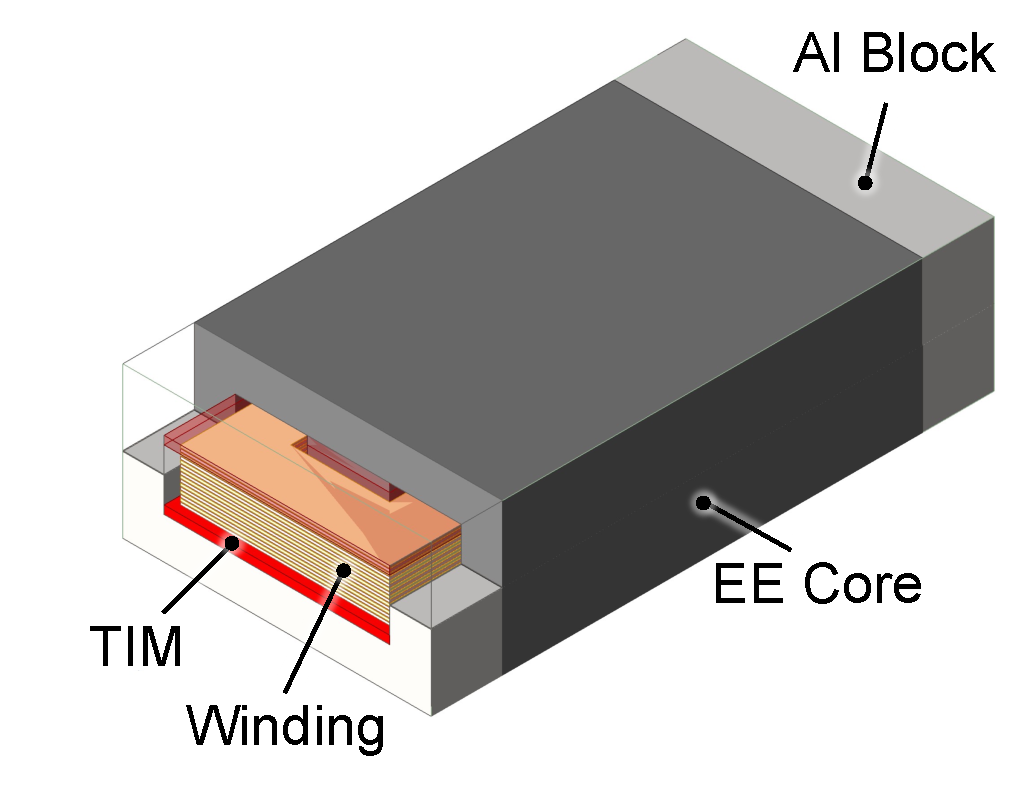
\includegraphics[width=0.5\columnwidth]{figures_chapter4/edgewise_simmodel.pdf}%
        \label{fig:sim_model_edgewise}
    }
    \subfloat[]{
        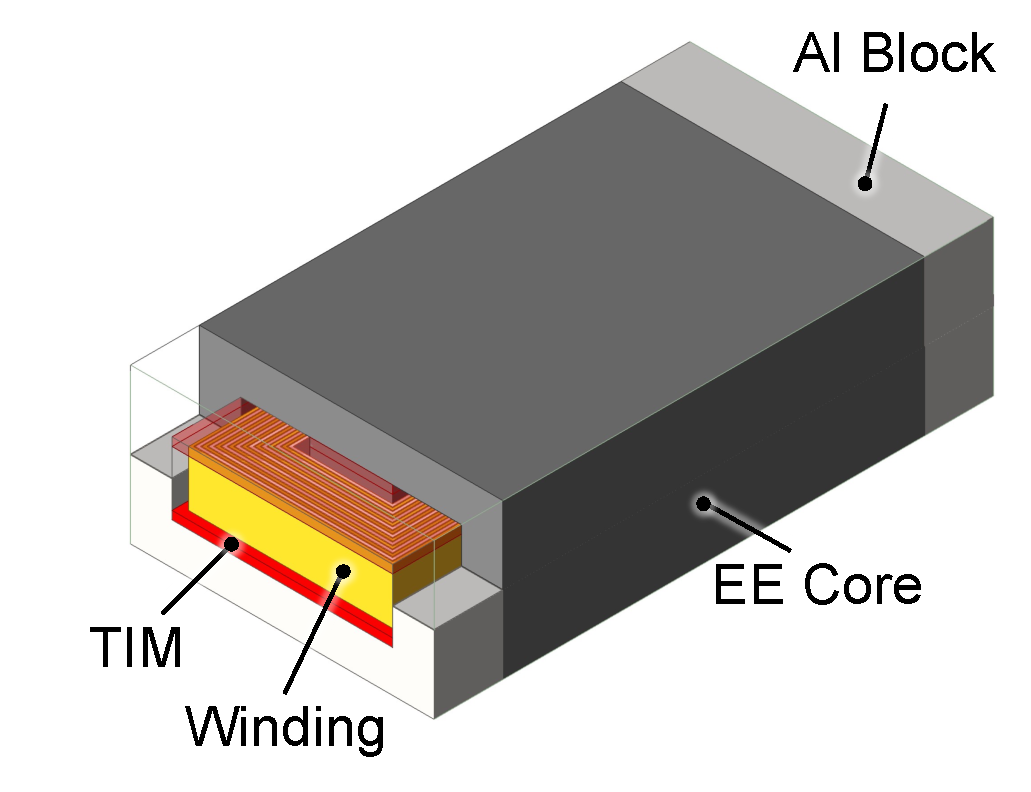
\includegraphics[width=0.5\columnwidth]{figures_chapter4/flatwise_simmodel.pdf}
        \label{fig:sim_model_flatwise}
    }
    \caption{Simulation models used of the (a) edgewise-wound (conventional) and (b) flatwise-wound (proposed) transformers.}
    \label{fig:simmodels}
\end{figure}

It is to be noted that the electromagnetic losses were coupled one-way into Ansys Icepak for the steady-state thermal analysis. This unidirectional coupling was deliberately selected to maintain a straightforward comparative baseline. While ferrite core losses are temperature-dependent, this characteristic varies significantly among different materials and introduces unnecessary complexity for a relative evaluation. 

\subsection{Electrostatic Simulation Conditions}
Electrostatic simulation using Ansys Maxwell was performed to evaluate if the transformer will avoid breakdown in operating conditions. To evaluate the isolation performance, designers set the secondary side voltage to 0 V (grounded) and assign a test DC voltage according to industry standard. Since the transformers in this study are a small-scale version of their counterparts, test voltages of 100 V and 200 V are applied to the primary side. The Electrostatic Solver was used for this set of simulations. A 2D simulation was utilized in this context since the transformer facial profile is symmetric around its geometry. The model used in the setup is shown in Figure \ref{fig:v_edge}a and \ref{fig:v_flat}a for the edgewise and flatwise configurations respectively.

\subsection{Thermal Simulation Conditions}
Steady-state Thermal simulation using Ansys Icepak was performed to evaluate the 3D steady-state spatial temperature distribution of the transformers. Two distinct thermal scenarios were evaluated. The losses from the electromagnetic simulation are coupled to their corresponding parts. First, natural air cooling was simulated to assess the intrinsic thermal performance of each transformer. This simply meant not applying any convection boundaries to the surfaces. Second, a forced air cooling scenario was modeled to represent practical operating conditions where the largest surface area of the transformer is mounted on a heat sink. This was implemented by applying a convective heat transfer coefficient of $h=$ 50 W/$(\text{m}^2\cdot K)$ to the bottom face of an aluminum block. The ambient temperature is set at 25.0$^\circ$C. The silicon-based TIM between the core and the windings has a thermal conductivity of 10 W/$(\text{m}\cdot K)$. A TIM with the same conductivity is also added as an interface between the bottom face of the transformer and the aluminum block. An example simulation model for the forced-air cooling setup is shown in Figure \ref{fig:forced_airsetup}.

\begin{figure}[h!]
    \centering
        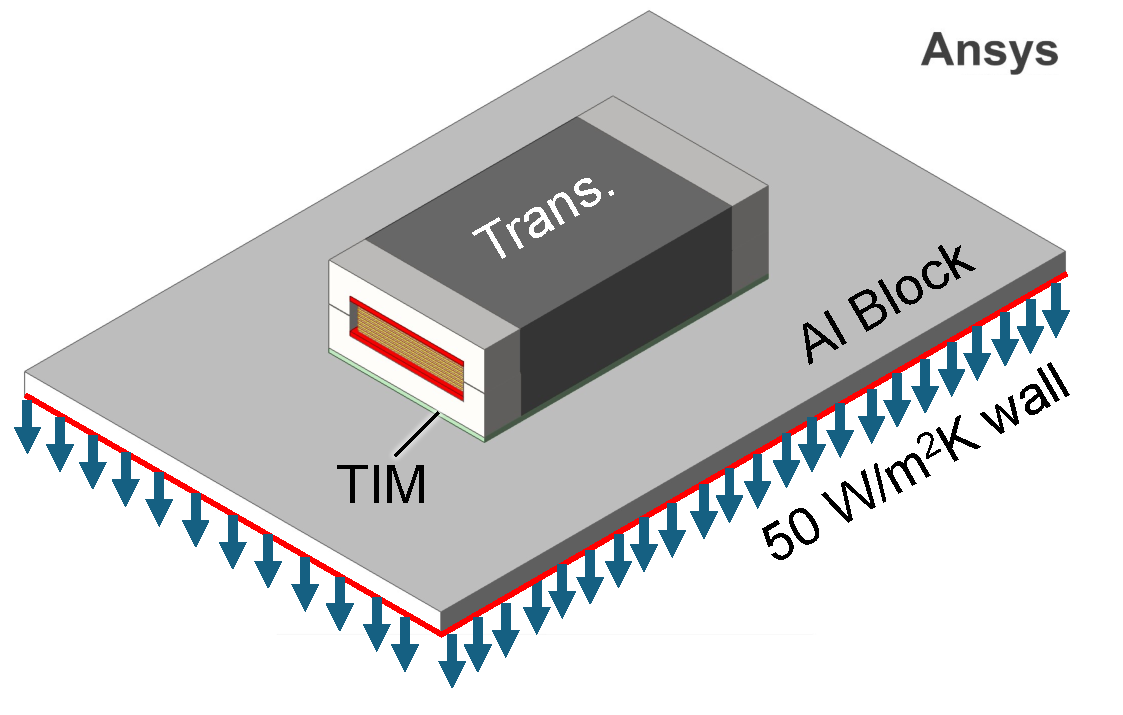
\includegraphics[width=0.5\columnwidth]{figures_chapter4/simsetup_forcedair.pdf}%
    \caption{Simulation model for the forced-air cooling scenario, as demonstrated on the edgewise-wound transformer.}
    \label{fig:forced_airsetup}
\end{figure}

\section{Simulation Results}

\subsection{Electromagnetic Simulation Results}
The electromagnetic simulation results at the operating frequency of 28.5 kHz are presented in Figure \ref{fig:bj_edge}a and Figure \ref{fig:bj_flat}a respectively. A close-up of the Magnetic Flux Density $B$ plots are shown in Figure \ref{fig:bj_edge}b and Figure \ref{fig:bj_flat}b respectively. A close-up of the Current Density $J$ plots are shown in Figure \ref{fig:bj_edge}c and Figure\ref{fig:bj_flat}c.

\begin{figure}[h!]
    \centering
        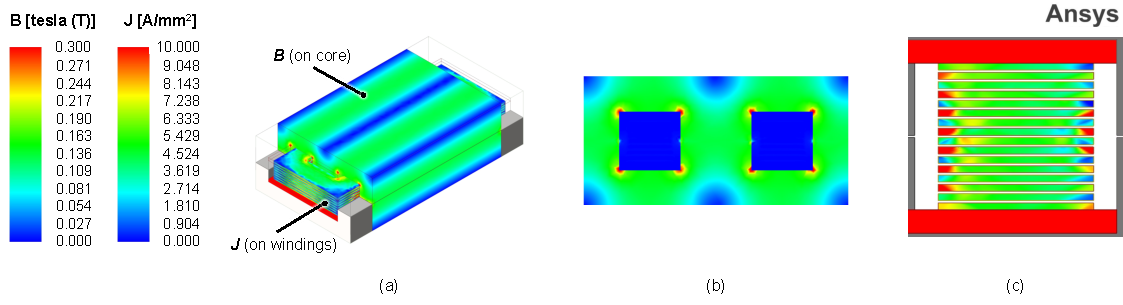
\includegraphics[width=\columnwidth]{figures_chapter4/bj_simresults_edgewise.pdf}%
    \caption{Electromagnetic simulation results for the edgewise-wound transformer: (a) $B$ and $J$ plots together, (b) close-up of $B$ plot, and (c) close-up of $J$ plot.}
    \label{fig:bj_edge}
\end{figure}

\begin{figure}[h!]
    \centering
        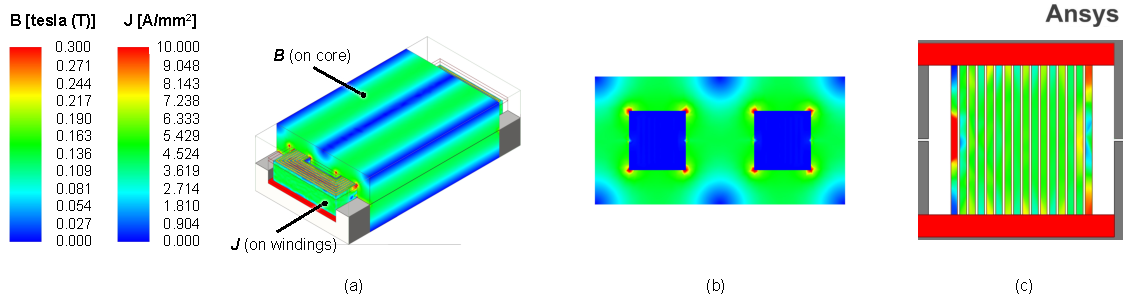
\includegraphics[width=\columnwidth]{figures_chapter4/bj_simresults_flatwise.pdf}%
    \caption{Electromagnetic simulation results for the flatwise-wound (proposed) transformer: (a) $B$ and $J$ plots together, (b) close-up of $B$ plot, and (c) close-up of $J$ plot.}
    \label{fig:bj_flat}
\end{figure}

The obtained magnetizing inductances are 200.14 $\upmu$H and 200.93 $\upmu$H for the edgewise and flatwise-wound transformers respectively, validating the $L_m$ design given the chosen parameters. The expected behaviors of the Magnetic Flux Density $B$ are seen and both transformers are not saturated. Moreover, the current density distribution is also expected, as current tends to crowd where the H-field is more prominent, which is towards the air gaps.  

\subsection{Electrostatic Simulation Results}\label{sec:breakdown}
The electrostatic simulation setups for the edgewise-wound and flatwise-wound (proposed) transformers are shown in Figure \ref{fig:v_edge}a and Figure \ref{fig:v_flat}a respectively. A 2D cross-section representing one window is taken as the simulation environment. The electric-field $E$ plots at 100 V test voltage are shown in Figure \ref{fig:v_edge}b and Figure \ref{fig:v_flat}b for the edgewise-wound and flatwise-wound transformers respectively. The $E$ plots at 200 V test voltage are shown in Figure \ref{fig:v_edge}c and Figure \ref{fig:v_flat}c for the edgewise-wound and flatwise-wound transformers respectively. As seen from the $E$ plots, the chosen $d_\mathrm{inter}$ is able to stand up to 200 V without causing electrical breakdown. There are some hotspots towards the intersection of air and the wires, and also at the triple point of the air, TIM, and the wire, but these do not reach the threshold.  

\begin{figure}[h!]
    \centering
        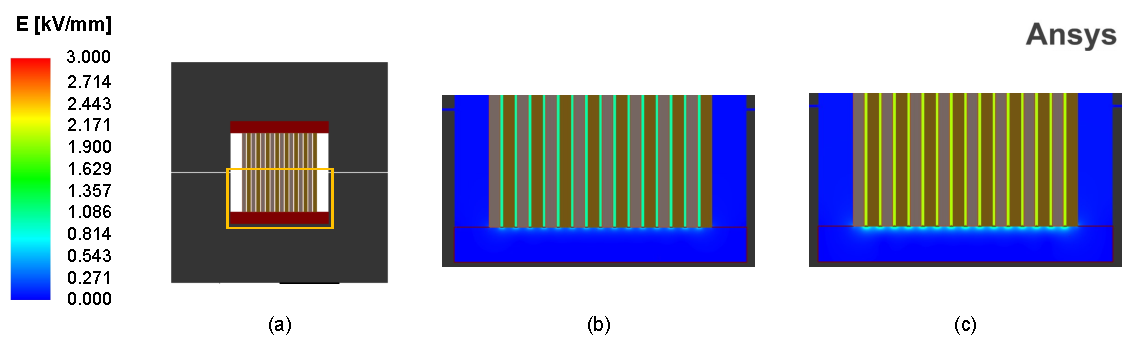
\includegraphics[width=\columnwidth]{figures_chapter4/efield_simresults_edgewise.pdf} 
    \caption{Electrostatic simulation (a) setup and results for the edgewise-wound transformer: (b) 100 V test voltage, and (c) 200 V test voltage.}
    \label{fig:v_edge}
    
\end{figure}

\begin{figure}[h!]
    \centering
        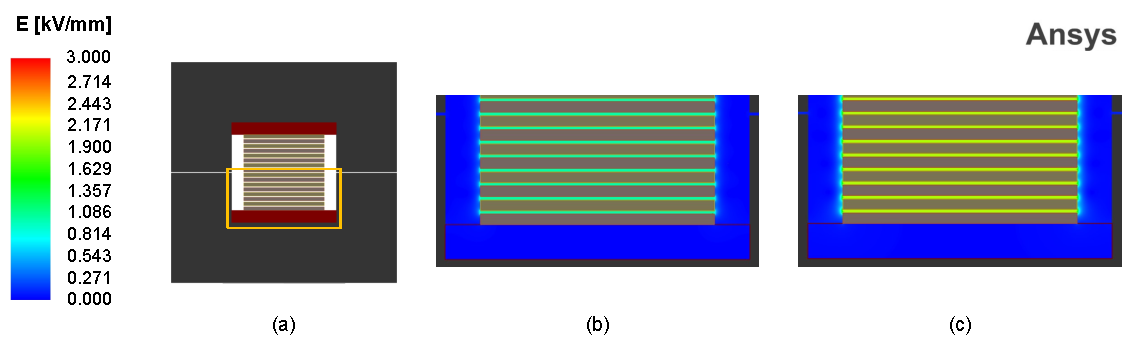
\includegraphics[width=\columnwidth]{figures_chapter4/efield_simresults_flatwise.pdf}
    \caption{Electrostatic simulation (a) setup and results for the flatwise-wound (proposed) transformer: (b) 100 V test voltage, and (c) 200 V test voltage.}
     \label{fig:v_flat}
    
\end{figure}

\subsection{Thermal Simulation Results} 
The thermal simulation results at the operating frequency of 28.5 kHz are presented in Figure \ref{fig:temp_natural}. Under the natural cooling scenario, the edgewise-wound transformer, as shown in Figure \ref{fig:temp_natural}, confirms the predicted thermal bottleneck; the inefficient series thermal path leads to localized heat accumulation in the windings, resulting in a significantly higher peak temperature of 66.9$^\circ$C. In contrast, the proposed flatwise-wound transformer, as shown in Figure \ref{fig:temp_natural}b, demonstrates superior thermal stability, exhibiting a uniform heat distribution and a peak temperature of approximately 56.0$^\circ$C. This discrepancy confirms that the flatwise structure offers a lower internal thermal resistance, thereby validating the heat extraction principles discussed in Section \ref{section:heat_dissipation}.

\begin{figure}[h!]
    \centering
        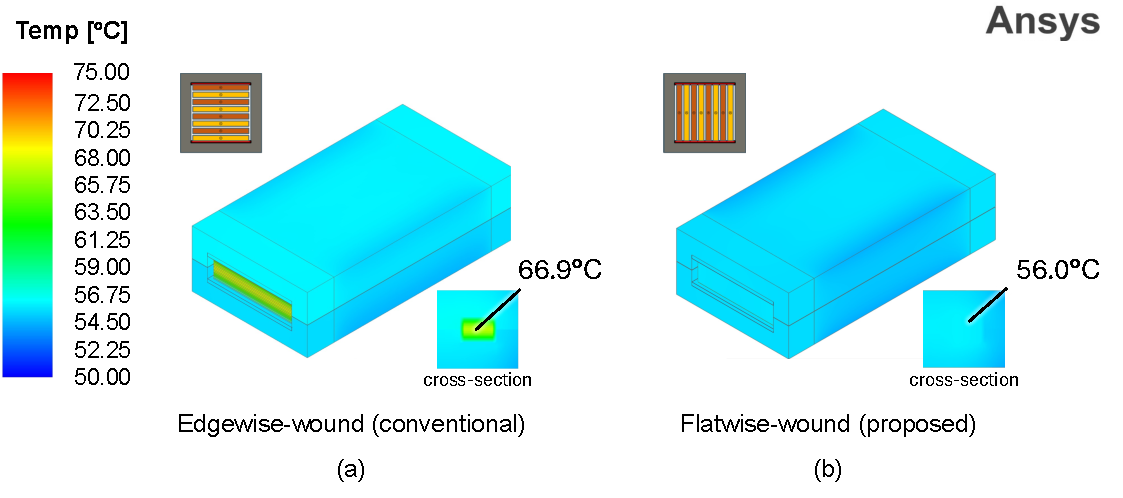
\includegraphics[width=\columnwidth]{figures_chapter4/natural_simresults.pdf}%
    \caption{Thermal simulation results of the (a) edgewise-wound and (b) flatwise-wound (proposed) transformers examined at 28.5 kHz, under natural cooling, at 25.0$^\circ$C ambient temperature.}
    \label{fig:temp_natural}
\end{figure}
The forced-air cooling scenario further amplifies this advantage. The edgewise-wound transformer as shown in Figure \ref{fig:temp_forced}a, continues to exhibit heat trapping within the central winding layers, resulting in a peak of 43.6$^\circ\text{C}$. Conversely, the flatwise model as shown in Figure \ref{fig:temp_forced}b, maintains a remarkably low peak temperature of approximately 30.2$^\circ\text{C}$ with a uniform gradient. These results highlight the scalable thermal advantage of the flatwise structure, demonstrating its effectiveness when integrated with practical cooling schemes. 

\begin{figure}[h!]
    \centering
    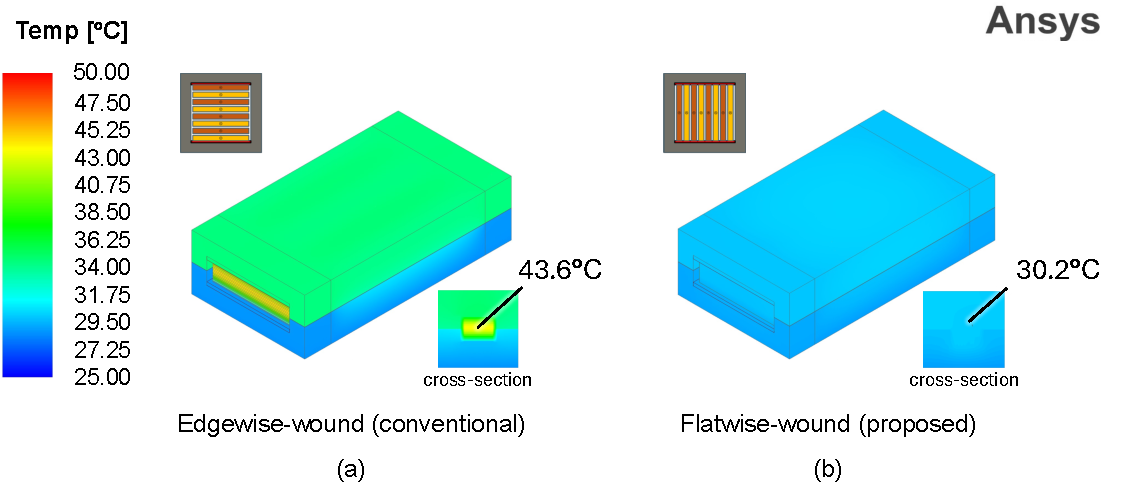
\includegraphics[width=\columnwidth]{figures_chapter4/forced_simresults.pdf}%
    \caption{Thermal simulation results of the (a) edgewise-wound and (b) flatwise-wound (proposed) transformers examined at 28.5 kHz, under forced-air cooling, at 25.0$^\circ$C ambient temperature.}
    \label{fig:temp_forced}
\end{figure}

\subsection{Electrical Properties and Losses}
The electrical properties derived from the simulation are summarized in Table \ref{tab:loss_comparison}. The comparison demonstrates that both winding configurations exhibit highly comparable electrical characteristics. The flatwise structure incurs only a marginal increase in winding loss (2.33 W vs. 2.24 W) and interwinding capacitance (1.72 nF vs. 1.45 nF) compared to its edgewise counterpart. Despite this very small penalty in total power loss ($+$2.5\%), the flatwise structure achieves a drastically lower peak temperature and uniform heat distribution capability, demonstrating that the benefit of reduced internal thermal resistance far outweighs the minor increase in electrical loss. More characterization on the effect of each configuration to the parasitics is a highly recommended next step of the research.

\begin{table}[H]
    \caption{Electrical Properties and Losses of the Simulated Transformers}
    \centering
    % Auto-fits table to column width
    
        \begin{tabular}{ccccc}
            \hline
            \textbf{Parameter} & \textbf{Symbol} & \textbf{Flatwise (prop.)} & \textbf{Edgewise} & \textbf{Unit} \\
            \hline \hline
            Interwinding Capacitance & $C_{\mathrm{ps}}$ & 1.72 & 1.45 & nF \\
            Leakage Inductance & $L_{\mathrm{lk}}$ & 0.04 & 0.02 & $\upmu$H \\
            \hline
            Core Loss & $P_{\mathrm{core}}$ & 0.87 & 0.87 & W \\
            Winding Loss & $P_{\mathrm{wind}}$ & 2.33 & 2.24 & W \\
            Aluminum Loss & $P_{\mathrm{Al}}$ & 0.09 & 0.09 & W \\
            \textbf{Total Loss} & \textbf{$P_{\mathrm{total}}$} & \textbf{3.29} & \textbf{3.21} & \textbf{W} \\
            \hline
        \end{tabular}%
    
    \label{tab:loss_comparison}
\end{table}